

\documentclass{book}

\usepackage{geometry}
\usepackage{fancyhdr}
\usepackage{amsmath, amssymb}
\usepackage{graphicx}
\usepackage{color}
\usepackage{amssymb}
\usepackage{color}
\definecolor{bg}{rgb}{0.89, 0.95, 0.71} % background e3f3b4
\definecolor{ac}{rgb}{0.50, 0.18, 0.41} % accent c491b6
\definecolor{rc}{rgb}{0.77, 0.57, 0.71} % rule 7f2f69

\usepackage{url}
\usepackage[pdftex, 
            bookmarks, 
            colorlinks=true,
            linkcolor=black, 
            plainpages = false,
            pdfpagemode = UseNone,
            pdfstartview = FitH, 
            citecolor = ac, urlcolor = ac, filecolor = ac]{hyperref}


% \title{MICROPROCESSORS\\ \& \\ MICROCONTROLLERS}
% \author{Aurabindo J\\ \small{aurabindo@computer.org}}
% \date{\today}

\begin{document}
%\maketitle
%\thispagestyle{empty}	
%\newpage

\newcommand{\HRule}{\rule{\linewidth}{1mm}}

\begin{titlepage}

\vspace*{6cm}
\thispagestyle{empty}
\begin{center}
\HRule \\[0.4cm] { \Huge \textsc Microprocessors \& Microcontrollers}\\[0.4cm] \HRule \\[1.5cm]


\begin{center} {\large Aurabindo J} \\[.2cm] {\texttt aurabindo@computer.org}
\end{center} 



\vfill
{\large \today}

\end{center}


\end{titlepage}

\pagestyle{headings}
\setcounter{page}{1}
\pagenumbering{roman}

\section*{{\huge About the Book}}
\addcontentsline{toc}{section}{About the Book}



This book is specially written for the use of students of the Calicut University
for the course EE09-601 MICROPROCESSORS \& MICROCONTROLLERS. This is an
open-source project, done using \LaTeX .\\[.1cm]

\noindent The first chapter is not in the syllabus. But you should be thorough with that part if you want the preceeding chapters to really make some sense to you. If you plan to skip the first part, then there is no special benefit you get out of this book. Happy reading!!!
\\[4.5cm]

\begin{quote}

Copyright \copyright\ 2012 Aurabindo J\\[.3cm ]
This book is a free software; you can redistribute it and/or modify it
under the terms of the GNU General Public License as published by
the Free Software Foundation; either version 3 of the License, or
(at your option) any later version.

This book is distributed in the hope that it will be useful, but WITHOUT
ANY WARRANTY; without even the implied warranty of MERCHANTABILITY
or FITNESS FOR A PARTICULAR PURPOSE.  See the GNU General Public
License for more details.

\end{quote}
\pagebreak


% \newpage

\tableofcontents
\newpage

\setcounter{page}{1}
\pagenumbering{arabic}


\chapter{An informal Introduction}

You\rq ve been hearing the word \lq microprocessor\rq\ for quiet a long time.
Before we move on, i would like to quote that, microprocessors
are the most complex thing mankind has ever made. If you were to represent the
circuit diagram of a modern desktop processor like the Intel Core i7 on an A4
sheet, on a scale of 10 transisitors per page, you`ll need more than 20 million
sheets!!! To be precise, there are 2.27 billion transisitors, and that too in 434 $mm^2$ of area! The total population of the world is 7 billion. Not bad, the transisitor is closing in :-) Even the whole blueprint of burj khalifa wouldn\rq t take more that
500 sheets! Look around you. Try to enumerate a few things that did\rq nt need
any help of a microprocessor to make it look like the way it is. In almost
evrything you see, hear or use, is associated with a processor - whether
directly or indirectly. That means living in a world without a microprocessor is
same as living in the stone age! There is a one-liner which says, \lq\lq Behind
every successful man, there is a lady\rq\rq. Now, I would like to make a small
change to it: \lq\lq Behind every success, there is a processor\rq\rq!!! :-P

Now that processor based systems are inevitable part of our lives, its a shame
if we know nothing much in detail about it. There is a significant difference
between a pure electrical system, like a machinery, and a microprocessor
(obviously,
not the way you thought :-P). Consider the old days when Faraday invented that a
moving coil in a magnetic field created an EMF. Even if Faraday didn\rq t
invent that, that magnetic filed will definitely produce EMF in that coil. But
the
processor, on the other hand, was totally created by humans. That means if
someone didn\rq t invent it, then someone else must have invented it. Else, it
wont exist today. What i mean is that this little complex thing was created by
humans, and if you can learn all those complex stuff that the humans didn\rq t
create, then you can easily learn what a human created!

\section{Microprocessors and Microcontrollers}
Before you start leanring about $\mu$p and $\mu$c, you should know the differece
between a controller and a processor. You already know what a microprocessor is
-- the ones like Intel Core i7 , AMD Athlon, etc. To understand what a
microcontroller is, consider the components inside a CPU. There is a motherboard
which holds the important components like RAM, processor, BIOS, various ports
for input \& output, etc. So, if core i7 is the microprocessor, then the
motherboard is the microcontroller. But, a motherboard is never called a
microcontroller, as it is much more complex and general purpose thing. So when
we call something a microcontroller, it will be very small, and its capabilities
will be very much limited and fixed. To make it clear, a microcontroller is a
system
comprising of a microprocessor, the primary memory (similar to RAM), a firmware
(similar to BIOS), some input/output pins (similar to ports like USB, VGA, etc),
and many other additional stuff (Analog to Digital Converters, etc.), on a
single platform, say an IC (similar to the PCB of the motherboard).

\section*{The Pre-Requisites}

Inorder to learn how a $\mu$p works, you just need to know some digital
electronics -- stuff like flip flops, various types of registers (parallel load,
shift, counter, etc.). For a reference, use \emph{Digital Logic \&
Computer Design}, \emph{Computer System Architecture} both by \emph{Morris Mano}
and \emph{Computer Organization \& Design} by \emph{Patterson \& Hennesey}.


\section{How does a processor work ?}

Considering the complexity of a modern computer, it\rq s hard to explain how
your
Core i7 works at this point. So, we\rq ll first see the working of a really
basic $\mu$p. You know very well
that a $\mu$ p understands nothing other than a 0 \& 1. Yet it manages to do all
those
complex stuff. The key concept behind the\rq s working is it\rq s ability to
treat a group of
bits as\lq instruction\rq\ or \lq data\rq. The instruction tells the $\mu$p what
it
should do -- whether to do an addition, a logic operation, a memory read/write
operation, or whatever.
The same may instruction tell the $\mu$p to treat a group of bits as data and
operate on them. 

In essence, the only thing (this) $\mu$p does is, it continuously fetches some
binary
data from memory (which will be treated as instruction), decodes it so as to
understand what to do next, and then executes
it. It does this in sequence, not everything together. First it will read the
instruction from memory. It will then decode. At this point, it will understand
whether it has to fetch more bits, or to execute the instruction. After it
finishes the execution,
it will then go to the next memory location to fetch the next group ob bits,
which will be treated as instruction.

Consider a computer that has \lq\lq1000001010" stored in the very first address
of
the memory location \lq\lq0000". This is called the \lq instruction code\rq.
Consider that this instruction performs an addition of two numbers stored in two
register. So when the computer starts, 
it fetches the bits at "0000".  Basically, this can be divided into
two parts -- The Operation Code or the \lq OpCode\rq\ and data. This data may be
considered
as an operand or the \emph{address} of an operand. In the example code, the
first 4 bits, \lq\lq 1000" is the OpCode. The subsequent group of 3 bits, \lq\lq
001"
and \lq\lq 010" are called operands. Here, the OpCode specifies the ADD
instruction. The operands \lq\lq001" and ``010" will act as two register, say 
A (the accumulator) and B. In short, the above instruction is similar to
\texttt{ADD B} instruction in 8085. 

\subsection{Instruction Code Formats}
\label{n_byte_ins}
The instructions in a $\mu$p can be classified on different basis. Basically, we
can classify them into 3 categories:\\
\begin{tabbing}
\hspace{1cm}\= 	\begin{tabular}{|c|c|}
	
		\hline
		Operation Code & Address of Operand

		\hline 
	       \end{tabular} \= (c) Immedeate Operand\kill

	    \>	\begin{tabular}{|c|}
		\hline
		Operation Code \\
		\hline 
	       \end{tabular} \> (a) Implied \\ \\
	    \> \begin{tabular}{|c|c|}
		\hline
		Operation Code & Operand \\
		\hline 
	       \end{tabular} \>  (b) Immedeate Operand \\ \\
	    \> \begin{tabular}{|c|c|}	
		\hline
		Operation Code & Address of Operand \\
		\hline 
	       \end{tabular} \>  (c) Direct Address \\ \\
\end{tabbing}

Examples from 8051 for the implied categories include \texttt{HLT, XCHG}. As
they dont need any further information like additional operands, they can easily
fit inside a 1 byte instruction code. Consider the instruction \texttt{MVI A,
05h}.  This might need more space to accomodate all the information.
\texttt{MVI} might be represented by ``01010", A by "000" and 05h by itself
(00000101). So, it takes excatly 16 bits. Hence, its a 2 byte instruction.
Consider \texttt{LDA 2500h}. \texttt{LDA} takes 5 bits, and it accomodates the
remaining 16 bits of 2500h in the next 2 locations of 1 byte each. Hence, it\rq
s a 3 byte instruction.

\section{A Simple Computer}

The processor core of a computer is having a lot of registers. They may be
general purpose register, that the users (programmers) can read and write, or special registers
that only the processor can access. We shall see some of the basic registers
found in all processors.
\begin{itemize}
  \item \textit{Program Counter} \\[5pt]
    It\rq s simlpy a counter. It is perhaps the most important part of the
computer. It initiates the fetch operation. While the computer is powered on, PC
is reset to a value, say ``0000". The fetching circuit takes this output of PC
and goes to that memory location. After the execution is over, when the next
clock tick comes, the counter incrementes to ``0001". The fetch circuit again
does the same thing and this cycle continues. It is mandatory that the next
clock tick arrives only AFTER the current fetch is complete. Else, you wont get
the expected result as the next execution may depend on the vaules of the
current execution. The tiny elementary operations that a $\mu$p can do are
called \emph{micro operations}. A group of such operation that do a meaningful
operation is called a \emph{macro operation}
    \begin{quote}
    \textbf{A note for the Geeks:} You might have heard of processor overclocking. The maximum clock speed you can run your $\mu$p is the value limited by the
time it takes to complete one such cycle as mentioned above. So if you increase
the clock frequency too much, it will trigger an operation before an ongoing
operation is completed. This can have very adverse effects on the system, as the
operation being read cannot be predicted. In fact, it can be anything. It
may be corresponding to a memory erase operation. And if that happens to be on your
Master Boot Record, then, ``Govinda!!!". It can even burn out the processor -- ``Gooovindaaa!!!" :-P
    \end{quote}
  \item \textit{Memory Address/Buffer Register} \\[5pt]
    Memory Opeartions are the basic things any computer should do. For this
purpose, there are two register, MAR and MBR. During a read operation, the the
address that should be read is sent to the MAR. The MBR will hold the contents
of the memory word read from or written into memory.

  \item\textit{Instruction Register} \\[5pt]
  When an instruction is read from the memory, it is first placed in the MBR and
later to the IR. It decodes the OpCode of the instruction and provides a unique output for each instruction, similar to the \emph{one hot} assignment. Thus if $q_1=1$ if the OpCode is equivalent to binary 1, $q_2=1$ if OpCode is binary 2, and so on.

  \item\textit{Timing Counter} \\[5pt]
  This is an important component of a computer, but this is invisible to the programmer. It synchronizes the fetch, decode and execute cycles of the $\mu$p with the clock pulse. The clock pulse of a digital system is like what the heart beat is, for a human. From the input clock pulse, a set of phase shifted clock pulses are derived as shown in the figure. Each ouput of the derived clock pulse will be connected to a particular circuit which does a particular micro operation. 



  \item\textit{Registers} \\[5pt]
  There will be a lot of general \& special purpose registers in a $\mu$p. One such special register is the Accumulator, usually denoted as \lq A\rq. There may be other registers, like \lq R\rq,\lq B\rq, etc.

\begin{figure}[h]

\begin{center}
  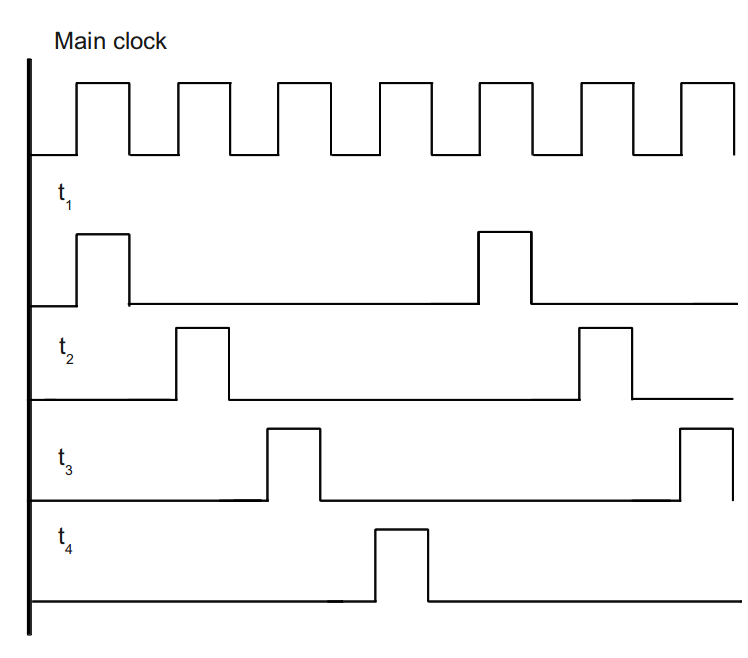
\includegraphics[scale=.35]{imgs/clock.png}
\end{center}
\caption{Timing Signals from Clock Pulses}
\end{figure}



The simple computer shown contains a memory unit, 7 registers \& 2 decoders. The memory unit stores an 8 bit data in a particular address. Eventhough all the data is stored in the memory, all the processing happens in the registers. The PC, IR, \& T are the part of the control unit. IR recieves the OpCode of instructions. The decoder supplies one output for each operation. The T counter is also decoded to supply eight timing variables $t_0$ thro\rq\ $t_7$ similar to the above figure. This counter is incremented every clock pulse (edge triggered). It can also be cleared at any time to start a new cycle.

\end{itemize}

\begin{figure}[h]

\begin{center}
  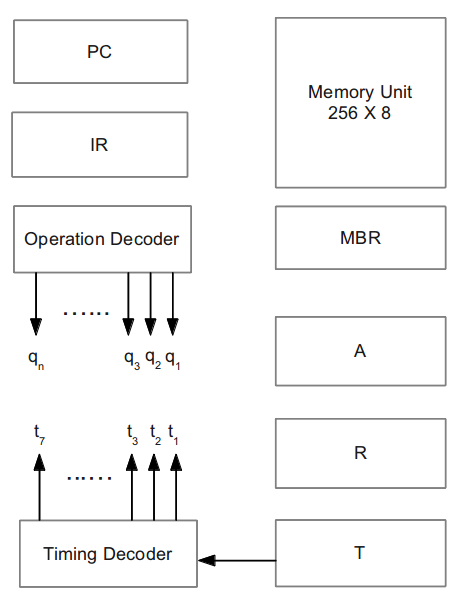
\includegraphics[scale=.60]{imgs/basic_comp.png}
\end{center}
\caption{Overview of a simple computer}
\end{figure}

The PC goes thro\rq\ a step-by-step counting sequence and causes the computer to read successive instructions previously stored in memory. The PC always holds the address of the next instruction in memory. To read an instruction, the contents of PC are transferred into MAR and a memory-read cycle us initiated. The PC is then incremented by 1 so that it holds the next address in the sequence of instructions. An OpCode read from memory into MBR is then transferred into IR. If the memory-address part of an instruction is read into MBR, this address is transferred into MAR to read the operand. Thus, MAR can recieve address either from PC or from MBR.

\subsection{Instruction Fetch Cycle}

The PC must be intialzed to contain the first address of the program stored in memory. Every processors have a \lq Power On Reset\rq\ that initializes the registers in it to some default value. When a \lq\lq Start\rq\rq\ switch is activated, the computer sequence follows a basic pattern. An OpCode whose address is in PC is read from memory into MBR. The PC is incremented by 1 to prepare it for the next address in sequence. The OpCode is transferred from MBR to IR, where it is decoded. This sequence is called the instruction fetch cycle, since it fetches the OpCode from memory and places it in a control register. In this example, the timing variables $t_0$, $t_1$ and $t_2$, out of the timing decoder are used as control functions to sequence the microoperations for reading an OpCode and place it into IR. It\rq s representation, called Register Transfer Language (RTL) is shown below:\\[.5pt]

\begin{tabular}{r l l}
$t_0$: & MAR $\leftarrow$ PC & Transfer OpCode Address \\
$t_1$: & MBR $\leftarrow$ M, PC $\leftarrow$ PC + 1 & Read OpCode, Increment PC\\
$t_2$: & IR $\leftarrow$ MBR & Transfer OpCode to IR\\
\end{tabular}
\\
\\
The timing counter T will start from the value 000 which produces a $t_0$ timing variable. The T register is incremented with every clock tick and automatically produces the next timing variables, $t_1$ , $t_2$, $t_3$, etc. in sequence. The first three timing variables execute the microoperation sequence which may be symbolized with the macrooperation statement $$ IR \leftarrow M[PC], PC \leftarrow PC + 1$$. This states that the memory word specified by the address in PC is transferred into IR and then the PC is incremented. The hardware constraint in the simple computer is that only MAR and MBR can access the memory. Since PC and IR cannot communicate directly with the memory, the above microoperation must be executed with a sequence of 3 microoperations. Another hardware constraint is that PC cannot be incremented when its value is being used to supply the address for a memory read. By transferring the contents of PC into MAR, the PC can be incremented while the memory reads the word addressed by MAR.

The fetch cycle is common to all instructions. This means that whenever a timing variable, $t_0$ through $t_2$ are in action, it will be a fetch cycle. The microoperations and control functions that follow the fetch cycle are determined in the control section from the decoded OpCode. This is available as outputs $q_i$, where $i = 1, 2, 3,...$. The 8085 has 246 instructions. Hence, the it internally has the decoded outputs $q_1$ through $q_{246}$. Latest x86 architectures have well above 1000 instructions.

\subsection{Execution of Instructions}

Execution start from the timing variable $t_3$, during which, the OpCode in IR and one output of the operation decoder is equal to 1. The control uses the $q_i$ variables to determine the next microoperations in sequence. Let \lq\lq MOV R\rq\rq\ instruction has an OpCode that makes $q_1 = 1$. The execution of this instruction requires the microoperation: $$q_1t_3:  A \leftarrow R, T \leftarrow 0$$
Thus when $q_1 = 1$ at time $t_3$, the contents of R are transferred into register A and the timing register T is cleared. by clearing T, the control goes back to the fetch cycle again to read the next instruction. Remember that PC was incremented during time $t_1$ so that it now holds the address of the very next instruction in sequence.

Now lets see how the LDI instruction is implemented. In 8 bit processors (like 8085), this instruction is stored by using two consecutive locations. (Refer section \S\ref{n_byte_ins} for more on instruction size and representation). Assume that this instruction is stored in memory like shown below:
\begin{center}
\begin{tabular}{r | l}
\textbf{Memory Address} & \textbf{Data}\\
\hline
01256 & .\\
01257 & ..\\
01258 & ...\\
01259 & 00010000\\
01260 & 11001010\\
01261 & ...\\
01262 & ..\\
01263 & .\\
\end{tabular}
\end{center}
The LDI OPRD instruction has an OpCode that makes $q_2=1$. The microoperations that execute this instruction are:
\\[.5cm]
\begin{tabular}{r l l}
$q_2t_3$: & MAR $\leftarrow$ PC & Transfer OpCode Address \\
$q_2t_4$: & MBR $\leftarrow$ M, PC $\leftarrow$ PC + 1 & Read Operand, Increment PC\\
$q_2t_5$: & A $\leftarrow$ MBR, T $\leftarrow$ 0 & Transfer Operand, go to fetch cycle\\
\end{tabular}
\\[.5cm]
The first two microoperations are excatly the same for a fetch operation, since this instruction wants to get the operand which is stored in the very next address. But the condition on the left side is different. Here, the value read from memory is considered as data. But in a fetch cycle, it was considered as an instruction and was transferred to IR. This time, it is transferred to the register A, as that is what LDI is supposed to do. Now the instruction is completely executed and therefore, the timing register has to be cleared so as to start the next fetch cycle. Again, note that PC was incremented during  $q_2t_4$ so that the current value in PC is that of the next instruction in sequence.

Now lets see how a 3 byte instruction (Indirect Addressing) is implemented. Consider \lq\lq LDA ADRS\rq\rq\ . This instruction has an OpCode which makes $q_3 = 1$. The required microoperations are:\\[.5cm]
\begin{tabular}{r l l}
$q_3t_3$: & MAR $\leftarrow$ PC & Transfer OpCode Address \\
$q_3t_4$: & MBR $\leftarrow$ M, PC $\leftarrow$ PC + 1 & Read Address of Operand, Increment PC\\
$q_3t_5$: & MAR $\leftarrow$ MBR & Transfer Operand address\\
$q_3t_6$: & MBR $\leftarrow$ M & Read operand\\
$q_3t_5$: & A $\leftarrow$ MBR, T $\leftarrow$ 0 & Transfer Operand to A, go to fetch cycle\\
\end{tabular}
\\[.4cm]
The address of the operand, symbolized by ADRS, is place in memory right after the OpCode. As PC was incremented during fetch cycle, it now holds the address of the operand we need. After microoperations during $t_4$, we get the address of the operand that is to be transferred to A. This address has to be given to the MAR again so that the memory puts the actual operand we need into MBR. We now have to increment PC so that it will point to the next instruction in the memory during the upcoming fetch cycle. Now the final value from MBR is transferred to the A register to complete the instruction. The timer is now cleared, which initiates the next fetch cycle when $t_0$ arrives.\\


The control functions and microoperations for the simple computer are summarized in table \ref{rtl_simple}. The first 3 timing variables constitute the fetch cycle which reads the OpCode into IR. The microoperations executed during $t_3$ depends on the OpCode value in IR. Either $q_1$,$q_2$ or $q_3$ can only be 1 at a time. Hence, only one of $q_1t_3$, $q_2t_3$ or $q_3t_3$ will occur at a time, since the control function is $q_x$ $\langle$ logical AND$\rangle$\ $t_3$.


\begin{table}[h,c]

\begin{center}
 \begin{tabular}{l r l}
 	\hline
 	FETCH & $t_0$: & MAR $\leftarrow$ PC \\
		  & $t_1$: & MBR $\leftarrow$ M, PC $\leftarrow$ PC + 1 \\
		  & $t_2$: & IR $\leftarrow$ MBR \\
	\hline
	MOV & $q_1t_3$: & A $\leftarrow$ R, T $\leftarrow$ 0 \\
	\hline
	LDI	& $q_2t_3$: & MAR $\leftarrow$ PC\\
		& $q_2t_4$: & MBR $\leftarrow$ M, PC $\leftarrow$ PC + 1 \\
		& $q_2t_5$: & A $\leftarrow$ MBR, T $\leftarrow$ 0\\
	\hline
	LDA & $q_3t_3$: & MAR $\leftarrow$ PC \\
		& $q_3t_4$: & MBR $\leftarrow$ M, PC $\leftarrow$ PC + 1 \\
		& $q_3t_5$: & MAR $\leftarrow$ MBR \\
		& $q_3t_6$: & MBR $\leftarrow$ M \\
		& $q_3t_7$: & A $\leftarrow$ MBR, T $\leftarrow$ 0\\
	\hline
  \end{tabular}
  \caption{\textbf{Register-transfer statements for simple computer}}
  \label{rtl_simple}
 \end{center}
\end{table}

\subsection{Design of computer}

A practical computer has many instructions. The one we are discussing is obviously not pretty useful, but by using only 3 instructions, the basic function of a digital computer can be clearly demonstrated. The list of microoperations specifies the types of registers and associated digital functions that must be incorporated in the system. The first step in the design is to scan the RTL listed in Table \ref{rtl_simple} and retrieve all the statements that perform the same microoperation on the same register. For example, MAR $\leftarrow$ PC is listed for $t_0$, $q_2t_3$, and in $q_3t_3$. These 3 lines are combined into one statement: $$t_0 + q_2t_3 + q_3t_3: MAR \leftarrow PC$$

{
  {\color{red} \textit{\huge The figure goes here. (Implementation of x1: MAR $\langle$ -- PC)} }
}

A control function is a boolean function. The + between te control functions denotes a Boolean OR operation and its absence denotes an AND operation. The hardware implementation uses the simplified equations: $t_0 + (q_2 + q_3)t_3$. The binary variable $x_1$ is applied to the load input of MAR and the outputs from PC are applied to the inputs of MAR. When $x_1 = 1$, the next clock pulse transfers the contents of PC to MAR. The binary variables that causes $x_1$ to be 1 comes from the operation and timing decoders in the control unit.

There are a total of 8 distinct microoperations for this computer. For each microoperation, the associated control functions are accumulated and OR'ed together as shown below:

\begin{table}[h,c]

\begin{center}
 \begin{tabular}{l  l}
  \hline
  $x_1 = t_0 + q_2t_3 + q_3t_3$: & MAR $\leftarrow$ PC\\
  $x_2 = q_3t_5$: & MAR $\leftarrow$ MBR\\
  $x_3 = t_1 + q_2t_4 + q_3t_4$: & PC $\leftarrow$ PC + 1\\
  $x_4 = x_3 + q_3t_4$: & MBR $\leftarrow$ M\\
  $x_5 = q_2t_5 + q_3t_7$: & A $\leftarrow$ MBR\\
  $x_6 = q_1t_3$: & A $\leftarrow$ R\\
  $x_7 = x_5 + x_6$: & T $\leftarrow$ 0\\
  $x_8 = t_2$: & IR $\leftarrow$ MBR\\
  
	
  \hline
  \end{tabular}
  \caption{\textbf{Hardware specifications for a simple computer}}
  \label{control_design}
 \end{center}
\end{table}

  {\color{red} \textit{\huge The big figure here} }


\chapter{Architecture of Intel 8086 \& Pentium}
This chapter explains the overall architecture of the Intel`s 8086 and Pentium
processors, its operations and
the interrupts in 8086.


\chapter{Assembly Language Programming}
---TO DO---
\chapter{Interfacing Peripherals with 8086}
---TO DO---
\chapter{The Intel 8051 Microcontroller}
---TO DO---
\end{document}
